\documentclass{standalone}
\usepackage{tikz}
\usepackage{ctex,siunitx}
\usepackage{tkz-euclide}
\usepackage{amsmath}
\usetikzlibrary{patterns, calc}
\usetikzlibrary {decorations.pathmorphing, decorations.pathreplacing, decorations.shapes,}
\begin{document}
\small
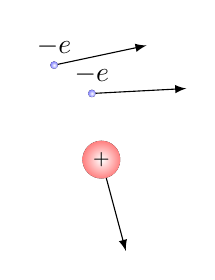
\begin{tikzpicture}[>=latex,scale=1.2]
  % \useasboundingbox(-0.5,-2)rectangle(8,6);
  \draw[->](0,1)--++(-75:1.0);
  \fill[inner color=white,outer color=red!50](0,1)circle(0.2)node{\scriptsize$+$};
  \draw[->](-0.1,1.7)--++(3:1.0);
  \draw[->](-0.5,2)--++(12:1.0);
  \fill[inner color=white,outer color=blue!50](-0.1,1.7)circle(0.04)node[above]{$-e$};
  \fill[inner color=white,outer color=blue!50](-0.5,2)circle(0.04)node[above]{$-e$};
\end{tikzpicture}
\end{document}